\section{Durchführung}
\label{sec:Durchführung}

In dem Versuch werden unterschiedliche Modelle mit dem Impuls-Echo-Verfahren 
untersucht. Dafür wird ein Ultraschallechoskop mit Ultraschallsonde verwendet, 
beides an einen Computer angeschlossen. Die Auswertung der Messdaten erfolgt
mit der Software EchoView, die sämtliche erforderlichen Scans durchführen kann.
Als Kontaktmittel werden bidestilliertes Wasser und Ultraschallgel genutzt.
\subsection{Acrylblock}
Zunächst wird ein Acrylblock wie in \autoref{fig:1} zu sehen, untersucht, 
einerseits mit der Schieblehre, darüber hinaus dann mit der Sonde. Das Bild 
ist von vorne aufgenommen, der Block verfügt über 11 Löcher mit ungleichen 
Radien, welche, wie auch deren Position im gesamten Block, mithilfe der 
Schieblehre vermessen werden.
\begin{figure}[H]
    \centering
        \centering
        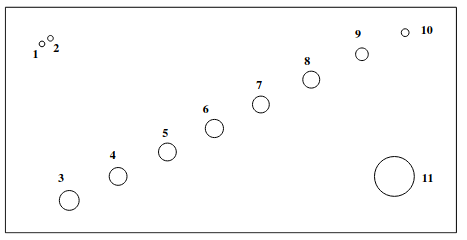
\includegraphics[width=0.7\textwidth]{Bilder/acrylblock.png}
        \caption{Frontansich des Acrylblocks.\cite{anleitung7}}
        \label{fig:1}
    \hfill
\end{figure}
\noindent Anschließend wird das bidestiliierte auf die Oberseite des Blocks 
gegeben und mittels der Sonde erfasst. Durch einen A-Scan werden die 
unterschiedlichen Laufzeiten der Schallwellen hin zu den Löchern gemessen.
Es ist zu beachten, dass auch die Beschichtung zwischen Acrylblock und Sonde 
einen Einfluss auf die Schallgeschwindigkeit hat. Jenes Verfahren wird analog 
für die Unterseite wiederholt.

\subsection{Augenmodell}
Bei dem Augenmodell wird als erstes vorsichtig etwas Ultraschallgel auf die 
Hornhaut des Auges aufgetragen. Im nächsten Schritt wird die Sonde aufgesetzt 
und das Impuls-Echo Verfahren kann beginnen. Der Einschallwinkel wird verändert 
bis die Echos von Iris, Linse und Retina durch Detektion von Intensität am 
Computer erkennbar sind. Aus den Laufzeiten des A-Scans können folglich die 
Abstände im Augapfel bestimmt werden.

\subsection{Brust mit Tumor}
Das vorliegende Brustmodell wird per Hand nach Tumoren untersucht, diese 
zeichnen sich durch verhärtetes Material bzw. Gewebe aus. Insgesamt gibt es 
zwei Tumore, die zu entdecken und untersuchen sind. Ist dieser Schritt 
absolviert, kommt es zur computertechnischen Erfassung, wobei ein A-und B-Scan 
an den Stellen mit den vermuteten Tumoren durchgeführt werden. Das geschieht 
möglichst linear und gleichmäßig. Darüber hinaus muss beachtet werden, die
Parameter im Programm auf Millimeter zu stellen, da Positionen der Tumore
bestimmt werden sollen. Als Kontaktmittel wird erneut Ultraschallgel verwendet.

\subsection{Herzmodell}
Als Herzmodell wird ein Plastikgefäß genutzt, welches in zwei Bereiche gegliedert 
ist, unten ein Hohlraum, welcher mithilfe einer Handpumpe mit Luft gefüllt 
werden kann. Darüber kann eine Flüssigkeit gefüllt werden. In diesem Experiment 
wird das Gefäß zu einem Drittel mit bidestilliertem Wasser gefüllt. Die 
Ultraschallsonde wird an die Wasseroberfläche gehalten. Dann kann der TM-Scan 
gestartet werden. Mithilfe der Pumpe werden Herzschläge simuliert, welche sich 
in der Grafik durch Hebungen und Senkungen bemerkbar machen sollen.